\documentclass[10pt,letterpaper,twocolumn]{article}

\usepackage[top=2.1cm,left=2.0cm,right=2.0cm,footskip=2.0cm]{geometry}
\usepackage[utf8]{inputenc}     % for Unicode
\usepackage{cite}               % citation
\usepackage[dvipdfmx]{hyperref} % links
\usepackage{caption}            % caption
\usepackage{microtype}          % improves typesetting in LaTeX
\usepackage{algpseudocode}
\usepackage{algorithm}
\usepackage{graphicx}
\usepackage{color} % ex.) \textcolor{color}{text}
\usepackage{url}

\renewcommand{\algorithmicrequire}{\textbf{Input:}}
\renewcommand{\algorithmicensure}{\textbf{Output:}}

\setcounter{topnumber}{100}
\setcounter{dbltopnumber}{100}
\renewcommand\topfraction{1.0}
\renewcommand\textfraction{0.0}
\renewcommand\dbltopfraction{1.0}
\renewcommand\dblfloatpagefraction{1.0}

\begin{document}

\twocolumn[
    \begin{flushleft}
        {\Large
        \textbf\newline{
            Periortree: An Extention of R-Tree for Periodic Boundary Conditions
            }
        }
        \newline
        \\
        Toru Niina \textsuperscript{1}
        \\
        \bigskip
        \bf{1.} Department of Biophysics, Graduate School of Science,
                Kyoto University, Kyoto 606-8502, Japan
        \\
        \bigskip
        * niina@theory.biophys.kyoto-u.ac.jp
    \end{flushleft}

    \section*{Abstract}
    Searching spatial data is an important operation for scientific simulations
    which are performed mostly on periodic boundary conditions.
    An R-Tree is a well known tree data structure used to contain spatial
    objects and it is capable of answering to spatial searching queries in an
    efficient way.
    In this paper, a novel method to construct an R-Tree considering periodic
    boundary conditions is presented.
    Unlike existing methods, the proposed method works without any kind of
    extra objects or queries.
    Moreover, because the method presented in this paper reduces the volume of
    bounding boxes for each nodes under the periodic boundary conditions,
    it is expected to increase the efficiency.
    This method is not only applicable to an R-Tree but also to other data
    structures that use axis-aligned bounding boxes and periodic boundary
    conditions.
    The implementation is available on GitHub.
    \bigskip
]

\section*{Introduction}

Computational simulations are essential tools for scientific research, such as
studying behaviors of complex biochemical models. To perform such large
scale simulations, both huge amount of computational resources and efficient
simulation softwares are required.

In most cases, searching for objects that satisfy some geometrical conditions
is one of the most time-consuming operation in a simulation. Generally, an
efficient algorithm that search objects drastically accelerates not only
the whole simulation processes, but also the data analysis of simulation results.
Therefore, a method that efficiently processes spatial search accelerates the
whole process of scientific simulation research.

An R-Tree is a widely used data structure representing bounding volume
hierarchies (BVH) by using an axis-aligned bounding box (AABB) for all its
entries~\cite{Guttman1984}.
It is capable of containing both sizeless and finite sized objects such as
points, segments, rectangles, spheres, etc.
In order to improve the efficiency, many variants of the R-Tree algorithm have
been proposed~\cite{Greene1989, Beckmann1990, Leuteneggert1997, Mitsuhashi2016}.

In order to use an R-Tree with periodic boundary conditions (PBCs), currently,
there exists two methods in the papers
(Figure~\ref{fig-method-rtree-pbc})~\cite{Mitsuhashi2016}.
The first method is described in Figure~\ref{fig-method-rtree-pbc}A.
It stores all the possible periodic images of the simulation system.
Because the periodic images are stored, it enables an R-Tree to
contain and search objects considering PBCs.
However, compared to a normal R-Tree, the memory consumption is increased
$3^D$ times (where $D$ reprecents a dimension of a system).
On the contrary, the other method (Figure~\ref{fig-method-rtree-pbc}B)
does not store periodic images.
When the query sticks out of the boundary, it replicates the query based on the
PBCs by transposing it periodically.
Although it works fine with points, it has a limitation when working with
finite-sized objects because it if query is inside of the boundary and objects
extend beyond the unit cell, some of them are overlooked
(Figure~\ref{fig-method-rtree-pbc}C).
One ad-hoc solution to overcome this limitation is changing the criteria for
replicating a query based on the size of elements that are contained.
This may increase the frequency in which queries are copied and decrease the
efficiency.

Here a novel method to construct and use an R-Tree with PBCs is proposed.
The main idea is to consider the PBCs when either entries are inserted or
objects are searched in an R-Tree.
By expanding an AABB and detecting intersection between AABBs under PBCs,
an R-Tree overcomes the limitation of containing finite-sized object with PBCs
(Figure~\ref{fig-method-rtree-pbc}D). Intersection and inclusion detection can be
implemented by introducing periodic transposition to the existing algorithms
with the appropreate representation of an AABB.
Consequently, this method requires the specific representation of an AABB.

This method does not require to copy objects or queries.
Moreover, using the information of the PBCs, it has more chance
to reduce the volume of AABBs of each node. Since the spatial
searching of an R-Tree is strongly affected by the volme of each node,
this feature may increase the efficiency.

\begin{figure}[hbt]
    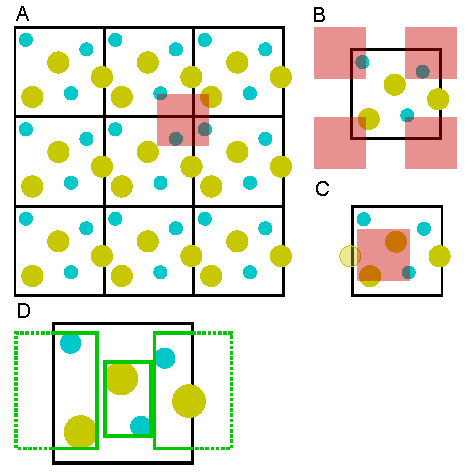
\includegraphics[width=8.4cm, bb=6 3 220 224]{fig1.eps}
    \caption{Methods to consider PBCs with R-Tree.
    (\textbf{A})
    By copying the unit cell, normal R-Tree can manage objects that are
    associated with periodic images.
    (\textbf{B})
    By copying query, R-Tree can find objects that are beyond boundary.
    (\textbf{C})
    With the method described in \textbf{B}, finite sized objects are
    overlooked when queries that is inside of the boundary are not copied.
    (\textbf{D})
    The method proposed in this paper. Forming AABBs according to
    the periodicity, R-Tree can organize objects under periodic boundary
    conditions.}
    \label{fig-method-rtree-pbc}
\end{figure}

The codes that are used in this paper are available on GitHub
(\url{http://github.com/ToruNiina/periortree}).

\section*{Methods}

Here some operations to modify and handle rectangles under PBCs are introduced.
Since the algorithm to grow and maintain the tree structure of an R-Tree is not
modified, it is not explained in this paper.
The fact that this method is independent from an R-Tree algorithm means that
the method can be applied to any R-Tree variant and to other spatial indexing
methods that are based on BVH and AABBs.

Because the rectangles used in R-Tree are axis-aligned, it is sufficient to show
an operation for one dimension. Applying it to each dimension successively,
these operations can be extended for higher dimension cases.

\paragraph{Representation of PBCs.}
Here, only cuboids are considered as the unit cell of the PBCs.
It is assumed that all the coordinates of the objects are restricted to be
inside of the unit cell.
There are well-known algorithm to restrict coordinates and inter-position
vectors to the unit cell.
In this paper, these algorithms are called as RestrictPosition and
RestrictVector, respectively.

\paragraph{Representation of AABBs.}
There are three common representations for AABBs
(Figure~\ref{fig-rectangle-rep})~\cite{real-time-collision-detection}.
The first one is a pair containing the minimum and maximum coordinate values
in each dimension.
The second one is a pair containing the minimum coordinate values and its width
in each dimension.
The third one is a pair containing the center position and the half-width
in each dimension.
Here, these are called as min-max, min-widths, and center-radius representation,
respectively.

Because the method proposed in this paper uses the center position of an AABB,
the center-radius representation is employed.
It is worth mentioning that this choice makes the implementation simpler,
but it is not indispensable.
Because all the representations have identical information about an AABB,
one can convert one representation to another.

\begin{figure}[thb]
    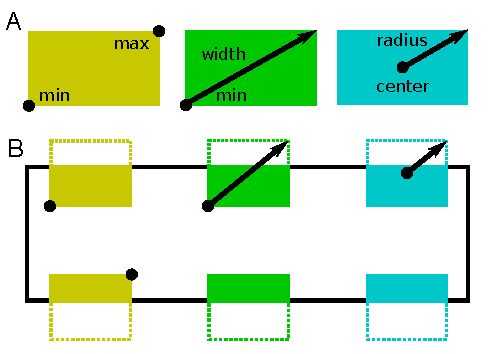
\includegraphics[width=8.4cm, bb=2 6 226 165]{fig-rect-rep.eps}
    \caption{
    (\textbf{A})
    Three popular representations of an AABB. The first one is min-max,
    the second one is min-widths, and the third one is center-radius representation.
    (\textbf{B})
    Three representations in a system with PBCs.
    The AABBs are colored in the same way as \textbf{A}.
    }
    \label{fig-rectangle-rep}
\end{figure}

\paragraph{Expanding AABBs according to PBCs.}
Expanding an AABB in order to contain a new object is one of the most
important operations in an R-Tree algorithm.
Because the total area covered by the AABB of each node affects the efficiency
of spatial searching, it is needed to find a way to make the area of the AABB
of each node as small as possible.

The algorithm to find the minimum expansion of AABB to contain another AABB
under PBCs is shown in Algorithm~\ref{expand_aabb_aabb}.
The size of a bounding box that contains two rectangles is determined by the
distance between their center points and their radius.
Therefore, by finding the minimum distance between the center points of the contents,
the minimum expansion is found. This can be accomplished by using RestrictVector.
When the contents are points, it is enough to find the minimum distance between
them(Algorithm~\ref{expand_aabb_point}).

\begin{algorithm}[tb]
    \caption{expand AABB to contain another AABB}
    \label{expand_aabb_aabb}
    \begin{algorithmic}
        \State $R1 \gets$ AABB to be expanded
        \State $R2 \gets$ rectangle to be contained
        \State $B  \gets$ boundary
        \Function{ExpandAABB}{$R1, R2, B$}
            \State $dc \gets R2.center - R1.center$
            \State $dc \gets$ \Call{RestrictVector}{dc, B}

            \State $l1 \gets R1.center - R1.radius$
            \State $u1 \gets R1.center + R1.radius$
            \State $l2 \gets (R1.center + dc) - R2.radius$
            \State $u2 \gets (R1.center + dc) + R2.radius$

            \State $L  \gets \Call{min}{l1, l2}$
            \State $U  \gets \Call{max}{u1, u2}$
            \State $C  \gets (L + U) / 2$
            \State $HW \gets (U - L) / 2$
            \State $C  \gets$ \Call{RestrictPosition}{C, B}

            \State \Return $\{C, HW\}$
        \EndFunction
     \end{algorithmic}
\end{algorithm}

\begin{algorithm}[tb]
    \caption{expand AABB to contain a point}
    \label{expand_aabb_point}
    \begin{algorithmic}
        \State $R \gets$ AABB to be expanded
        \State $P \gets$ point to be contained
        \State $B \gets$ boundary
        \Function{ExpandAABB}{$R, P, B$}
            \State $dc \gets P - R.center$
            \State $dc \gets$ \Call{RestrictVector}{dc, B}

            \State $l \gets R.center - R.radius$
            \State $u \gets R.center + R.radius$

            \State $L  \gets \Call{min}{l, P}$
            \State $U  \gets \Call{max}{u, P}$
            \State $C  \gets (L + U) / 2$
            \State $HW \gets (U - L) / 2$

            \State $C \gets$ \Call{RestrictPosition}{C, B}
            \State \Return $\{C, HW\}$
        \EndFunction
     \end{algorithmic}
\end{algorithm}

\paragraph{Finding an object based on BVH under PBCs.}

To find an object in an R-Tree, an algorithm that checks whether a
rectangle intersects another one or not is needed.
This can be determined by calculating the minimum distance between the centers of
the rectangles and then using the existing algorithm for the center-radius
representation(Algorithm~\ref{aabb_intersects_aabb}).
The inclusion can be detected in the same way
(Algorithm~\ref{aabb_within_aabb}, \ref{point_within_aabb}).

\begin{algorithm}[tb]
    \caption{Check whether an AABB intersects another AABB or not}
    \label{aabb_intersects_aabb}
    \begin{algorithmic}
        \State $R1 \gets$ rectangle
        \State $R2 \gets$ rectangle that might intersect to R1
        \State $B  \gets$ boundary
        \Function{IntersectsAABB}{$R1, R2, B$}
            \State $dc \gets R1.center - R2.center$
            \State $dc \gets$ \Call{RestrictVector}{dc, B}
            \State \Return \Call{abs}{dc} $\leq (R1.radius + R2.radius)$
        \EndFunction
     \end{algorithmic}
\end{algorithm}

\begin{algorithm}[tb]
    \caption{Check whether an AABB is inside of another AABB or not}
    \label{aabb_within_aabb}
    \begin{algorithmic}
        \State $R1 \gets$ rectangle
        \State $R2 \gets$ rectangle that might be inside of R1
        \State $B  \gets$ boundary
        \Function{IsAABBInsideOfAABB}{$R1, R2, B$}
            \State $dc \gets R1.center - R2.center$
            \State $dc \gets$ \Call{RestrictVector}{dc, B}

            \State \Return \Call{abs}{dc} $\leq (R1.radius - R2.radius)$
        \EndFunction
     \end{algorithmic}
\end{algorithm}

\begin{algorithm}[tb]
    \caption{Check whether a point is inside of an AABB or not}
    \label{point_within_aabb}
    \begin{algorithmic}
        \State $R \gets$ rectangle
        \State $P \gets$ point that might be inside of R
        \State $B \gets$ boundary
        \Function{IsPointInsideOfAABB}{$R, P, B$}
            \State $dc \gets R.center - P$
            \State $dc \gets$ \Call{RestrictVector}{dc, B}
            \State \Return \Call{abs}{dc} $\leq R.radius$
        \EndFunction
     \end{algorithmic}
\end{algorithm}

\section*{Results}

The steps of expansion of an AABB to contain rectangles is shown in
Figure~\ref{fig-result}A. There, the objects to be contained are colored
in black, and the AABB is colored in red.
It should be noted that, because it sticks out of the boundaries,
the periodic images of the bounding box are shown separately.

The last panel in Figure~\ref{fig-result}A shows that the proposed method
successfully finds a way to expand AABB with least enlargement under the PBCs.
Because the objects are distributed throughout the system,
if the AABB was expanded independently from the PBCs,
the AABB would wrap most of the area of the system.

In Figure~\ref{fig-result}B the results of queries are shown. It successfully
finds objects that are located beyond the boundaries. It should be noted
in the right panel of Figure~\ref{fig-result}B that because query box sticks out
of the boundary, the periodic images are shown separately.

\begin{figure}[tb]
    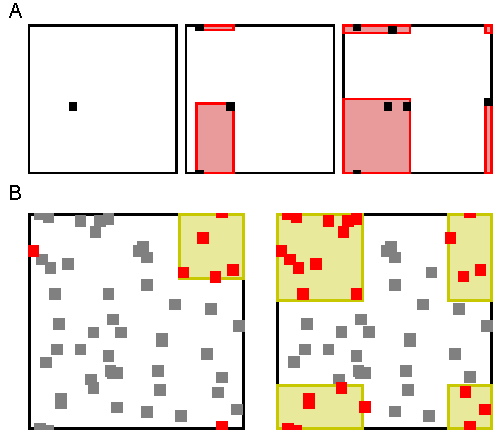
\includegraphics[width=8.4cm, bb=4 6 237 212]{fig-result-expand-intersect.eps}
    \caption{
    (\textbf{A})
    The three steps of expansion the AABB colored in red.
    It can be seen that the AABB is expanded beyond the boundary.
    (\textbf{B})
    The result of querying objects that intersect with the yellow rectangle.
    The objects contained in the R-Tree are shown as small square boxes
    and the ones intersecting the query box are colord in red.
    }
    \label{fig-result}
\end{figure}

\section*{Conclusion}

In this paper, a novel method for applying PBCs to R-Trees is introduced.
To detect intersection and inclusion, the existing methods for AABBs with
the center-radius representation can be used after applying periodic
transposition to AABBs.

This method is capable of containing not only points but also finite-sized
objects. It also removes the necessity of storing extra objects and
replicating queries. Moreover, it sometimes reduces the volume of each node
based on the boundary conditions.
On the other hand, since this method considers PBCs every time when AABBs are
expanded or checked whether it intersects another, it introduce tiny but
unavoidable computational costs into the whole process.

As described before, since this method modifies only the algorithms to expand an
AABB and to detect intersection between AABBs, it is applicable to other R-Tree
variants and to any spatial indexing method that works with AABBs.

Because the application of spatial indexing generally increase the performance
of spatiotemporal simulations, the proposed method might be useful for
scientific simulations under the PBCs.

\bibliographystyle{unsrt}
\bibliography{library}{}

\end{document}
